\documentclass[a4paper, 11pt, titlepage]{article}
\usepackage{fancyhdr}
\usepackage{graphicx}
\usepackage{imakeidx}
\usepackage{makeidx}
\usepackage{mathtools}
\usepackage[spanish]{babel}
\usepackage{eurosym}
\usepackage{hyperref}
\usepackage{amssymb}
\usepackage{listings}
\usepackage{xcolor}

\setcounter{secnumdepth}{5}
\setcounter{tocdepth}{5}

\title{Robustecimiento y securización SSH}
\author{Francisco Javier Balón Aguilar}

\begin{document}

\maketitle
\renewcommand{\contentsname}{Índice}
\tableofcontents
\newpage

\section*{Prólogo}
\newpage

\section{Introducción a SSH}

    SSH --o Secure Shell-- es uno de los protocolos más interesantes de los que se dispone 
    en la administración de sistemas, permitiendo acceder a otros equipos de forma remota; 
    pero sobretodo, de forma segura.
    
    Con SSH creamos un túnel entre cliente y servidor que simula, en la capa de aplicación, 
    la shell o intérprete de comandos del servidor, dotando al administrador de prácticamente 
    toda funcionalidad en el equipo.

    Generalmente se suele equiparar el protocolo SSH con el protocolo Telnet, ya que ambos 
    pretenden una funcionalidad similar. Aun así, existen diferencias notables, esencialmente 
    en la seguridad de las comunicaciones; ya que SSH utiliza técnicas criptográficas para 
    proteger los datos intercambiados entre ambos nodos que conforman la conexión SSH. SSH 
    utiliza un intercambio de claves basado en el protocolo criptográfico de \textit{Diffie-Hellman}, 
    imprescindible en el robustecimiento de la capa de transporte.

    Como vemos, SSH proporciona un sistema, a priori, seguro. Con una configuración con un 
    nivel aceptable de seguridad por defecto. Pero en función de la configuración del 
    servicio puede llevar al sistema a un estado de inseguridad. Por ello, es importante 
    entender el funcionamiento del protocolo, las funcionalidades que presenta y la configuración
    óptima en función de las necesidades del administrador. Este será el núcleo del presente 
    documento.

\section{Visión técnica del protocolo}

    Una vez introducido el protocolo, podemos arremangarnos y entrar en barro. El protocolo 
    SSH trabaja sobre el protocolo TCP/IP. Por ello, en primer lugar se realiza la conexión 
    TCP, realizando el \textit{three-way handshake}\footnote{
        \textit{Three-way handshake} o \textit{triple apretón de manos} es un método 
        utilizado en una red TCP/IP para crear una conexión entre un cliente local y 
        un servidor.

        Es un método de tres pasos en ambas direcciones simultáneamente diseñado para 
        permitir que ambos extremos de comunicación inicien y negocien los parámetros 
        de la conexión de socket TCP antes de que se transmitan datos.

        \[SYN, SYN+ACK, ACK\]
    }. Después de abrir la conexión, cliente y servidor se envían la versión disponible 
    del protocolo\footnote{
        Actualmente existen dos versiones del protocolo SSH; la versión 1 y la 2. La primera 
        es actualmente desaconsejable por motivos de seguridad, que son suplidos en la segunda 
        versión.
    }. Después, se utilizará el par de claves, pública y privada, de RSA. El servidor enviará 
    su clave pública de \textit{host} al cliente, de forma que éste pueda cifrar lo que necesite 
    enviar al servidor. El cliente comparará la clave pública de \textit{host} con la que 
    tenga almacenada del servidor en el archivo \textit{known\_host}, si lo hubiera. 

    \begin{figure}[htp]
        \centering
        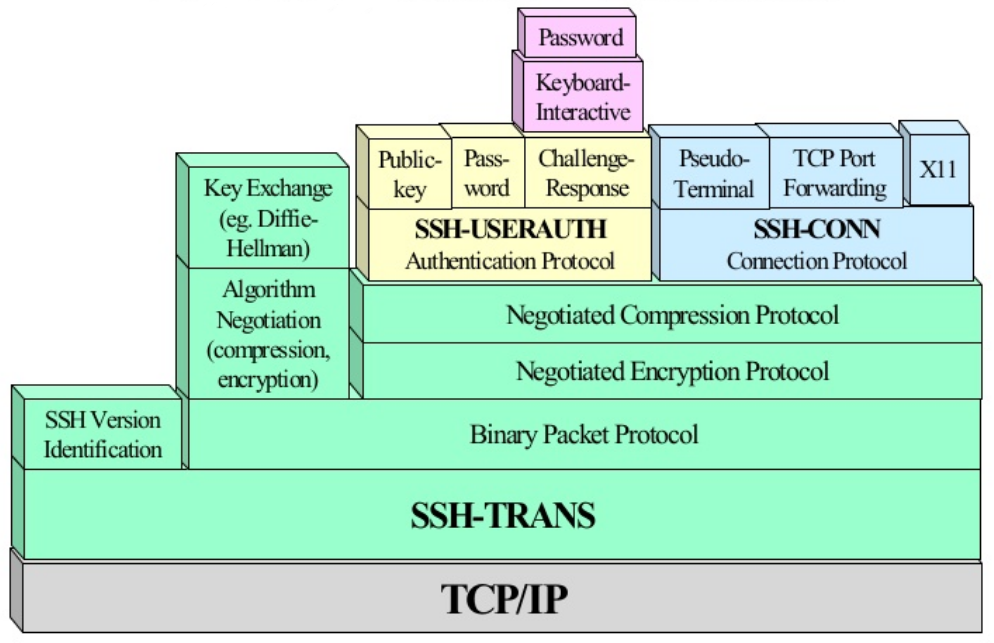
\includegraphics[width=0.8\textwidth]{resources/ssh00.png}
        \caption{Capas del protocolo SSH.}
        \label{ssh00}
    \end{figure}

    Una vez el cliente dispone de la clave pública del \textit{host} del servidor, este 
    generará una clave de sesión aleatoria y seleccionará un algoritmo de cifrado simétrico.
    Con esta clave de sesión, que se generará por defecto cada 3600 segundos, se cifrará el 
    túnel. El cliente enviará un mensaje que contiene la clave de sesión y el algoritmo de 
    cifrado seleccionado, información que viajará cifrada mediante la clave pública de \textit{host},
    al servidor. En este instante, el resto de la comunicación se utilizará el algoritmo de 
    cifrado simétrico y la clave compartida de sesión, dando velocidad a la conexión (en técnicas 
    de clave simétrica el cifrado y descifrado se hace más rápido), pero utilizando siempre 
    primero el protocolo de \textit{Diffie-Hellman} para poder enviar de forma segura 
    la clave compartida de sesión; y supliendo así la principal carencia en seguridad de los algoritmos 
    de criptografía simétrica: el intercambio de claves.

    Una vez tenemos el túnel creado, se llevará a cabo la autenticación del usuario en el 
    servidor, pudiendo utilizar distintos métodos para llevar a cabo tal autenticación.

\section{Instalación de servidor y cliente}

    La instalación tanto del cliente como del servidor es un proceso muy sencillo que no 
    ocupará mucho en la práctica. Debido que estamos utilizando la distribución Arch GNU/Linux, 
    utilizaremos el gestor de paquetes \textit{pacman}, en el que basa la distribución y que, 
    en código, no es más que una pantalla que realiza instalaciones de códigos fuentes \textit{tarballs}
    de forma automatizada. En caso de usar otra distribución, será necesario descargar el paquete 
    \textit{deb} (en aquellas distribuciones basadas en Debian) o \textit{rpm} (en aquellas distribuciones 
    basadas en Red Hat).

    \begin{figure}[htp]
        \centering
        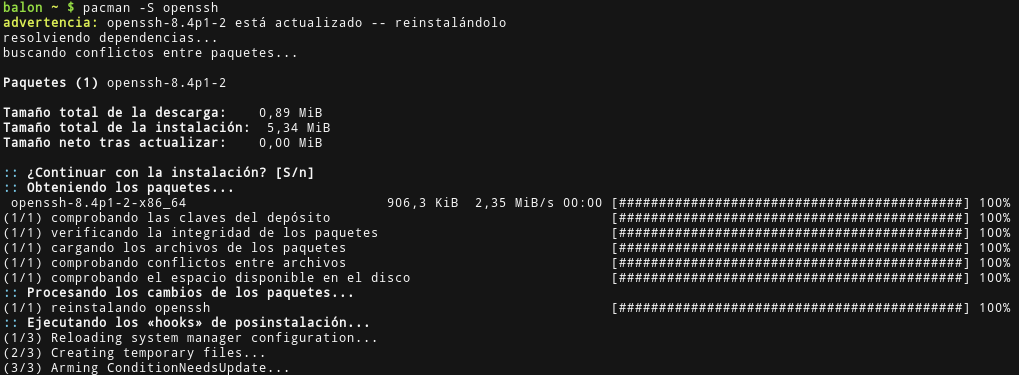
\includegraphics[width=1\textwidth]{resources/ssh01.png}
        \caption{Prueba de instalación de \textit{openssh} usando \textit{pacman}.}
        \label{ssh01}
    \end{figure}

    El paquete donde se encuentra es \textit{openssh}, que nació como alternativa libre a \textit{SSH 
    Communications Security} y que forma parte del proyecto OpenBSD.

\section{Configuración del servicio}

    Podemos clasificar la configuración de SSH en dos grupos: el directorio \textit{/etc/ssh} y el demonio 
    \textit{sshd}. El servidor o demonio cuenta con un fichero de configuración propio (\textit{/etc/ssh/sshd_config}), 
    mientras que el cliente cuenta con otro en el mismo directorio (\textit{/etc/ssh/ssh_config}).

    \subsection{Directivas básicas}
    \subsection{Autenticación básica con clave}
    \subsection{Autenticación mediante par de claves}
    \subsection{Proceso de conexión}
\section{Aplicaciones de SSH}
    \subsection{SCP}
    \subsection{SFTP}
    \subsection{SSHFS}
    \subsection{X11 forwarding}
    \subsubsection{Fail2ban}
\section{Tunneling}
    \subsection{Túneles TCP/IP con port forwarding}
\section{SOCKS}

\end{document}